\documentclass[11pt]{article}
\bibliographystyle{siam}
\usepackage{graphicx}

\title{Reproducing the Analysis of A High-Resolution 7-Tesla fMRI Dataset from 
Complex Natural Stimulation with an Audio Movie}
\author{
  Daks, Alon\\
  \texttt{alondaks}
  \and
  Yu, Lisa Ann\\
  \texttt{lisaannyu}
  \and
  Luo, Ying\\
  \texttt{yingtluo}
  \and
  Chang, Jordeen\\
  \texttt{Jodreen}
}

\begin{document}
\maketitle


\textbf{Paper:} Hanke, Michael, et al. "A High-Resolution 7-Tesla fMRI Dataset 
from Complex Natural Stimulation with an Audio Movie." Scientific data 1 (2014).
\newline
\newline    
\indent Most fMRI studies use highly simplified stimulus that are vastly 
dissimilar from what people experience in everyday life.  Hanke et al. sought to
create a
dataset of naturally occurring brain states by exposing participants to a 
more complex stimulus, the audio description of Forrest Gump.  This particular
audio description allows for the study of auditory attention and cognition, 
language and music perception, and retrieval of explicit memory without the
effect of visual imagery.  In addition, this dataset uses inter-individual 
synchronicity to study responses to complex processing.  This paper explains
the preparation of the dataset, such as collecting physiological information
then accounting for it in the voxels, and an initial analysis.  Hanke et al.
used representational similarity analysis to identify similar patterns
across brains.  They created a representationaly consistency map using pairwise
correlations.  After thresholding, the map revealed two clusters in the PT,
which is known to be used for auditory cognition.

The data is curated and segmented into 20 .TGZ files, where each of the 20 .TGZ 
files corresponds to one of the 20 subjects in the experiment. Each subject 
accounts for approximately 16 GBs of data. We verified the usability of the data
by inspecting and loading data corresponding to subject 1. We limited our 
initial exploration to a single subject since downloading each .TGZ takes 
approximately one hour. To ensure speedy access to the overall dataset when we 
begin central project work, our strategy for getting all the data entails each 
group member spending five hours downloading a different quarter of the overall
dataset, and then locally transferring the remaining three-quarters of the data
from our harddrives. Each subject's data includes several formats: subject
metadata(CSV), Raw BOLD functional MRI, Raw BOLD functional MRI 
(with applied distortion correction), Raw BOLD functional MRI (linear anatomical
alignment), Raw BOLD functional MRI (non-linear anatomical alignment), along 
with several Structural MRI datasets. The corrected and aligned versions of the
data attempt to eliminate device and scan related noise. Scan data is 
accessible in nibabel compatible formats (.NII).

Using nibabel, Matplotlib, and appropriate NumPy array slicing, we were able to
successfully load and display various brain images. The images appearing at the
end of the proposal are all taken from the central slice of their first
respective volumes.

The main purpose of the paper's experiment was to study properties of brain
response
patterns that are supposedly common when people are exposed to audio and movie
simulation. We intend to replicate their experiment using the data they gathered
from the 20 participants. For example, a BOLD time-series similarity measure
(e.g. correlation) is often used to quantify similarities in responses among
individuals. Hank et al. recognized that this was a common approach, but they
went beyond that and also implemented representational similarity analysis 
(RSA). To do so, we will create dissimilarity matrices for 18 individuals using
the same
searchlight mapping approach that they used (Subjects 4 and 10 were not included
due to missing data). Doing so will capture 2nd-order isomorphisms in response
patterns. Lastly, to access statistical significance, we will transform the
representational consistency map into percent rank with respect to the total
distribution of the DSM correlations. We'll calculate the mean correlation
coefficient and compare our value to theirs.
\begin{figure}[h]
\caption{Image from Raw Data}
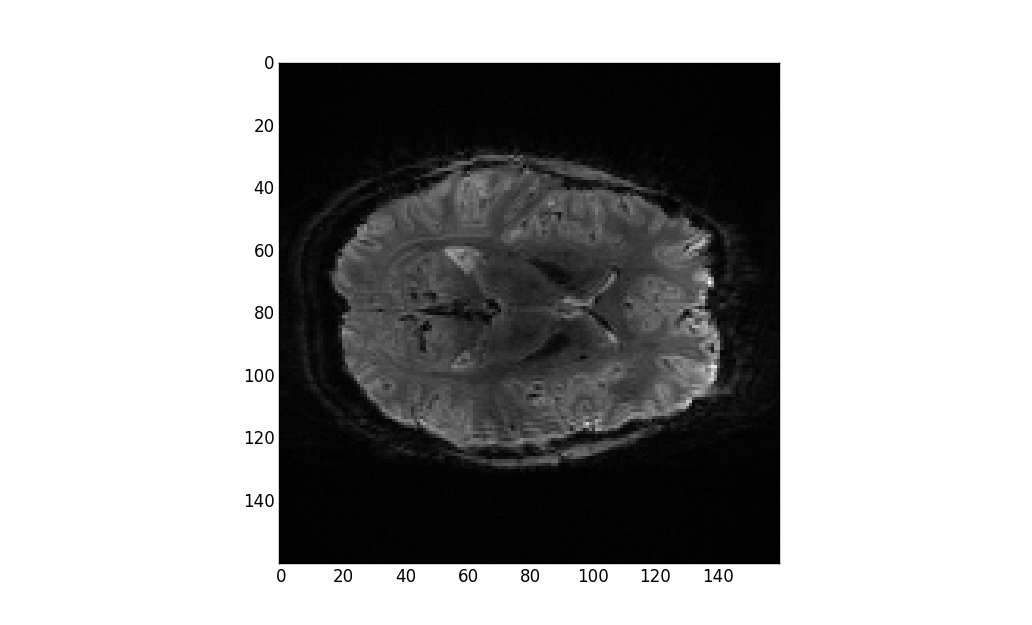
\includegraphics[scale=.5]{image_1}
\centering
\end{figure}
\begin{figure}[h]
\caption{Identical to raw BOLD image above, but with a scanner-side correction
for geometric
distortions}
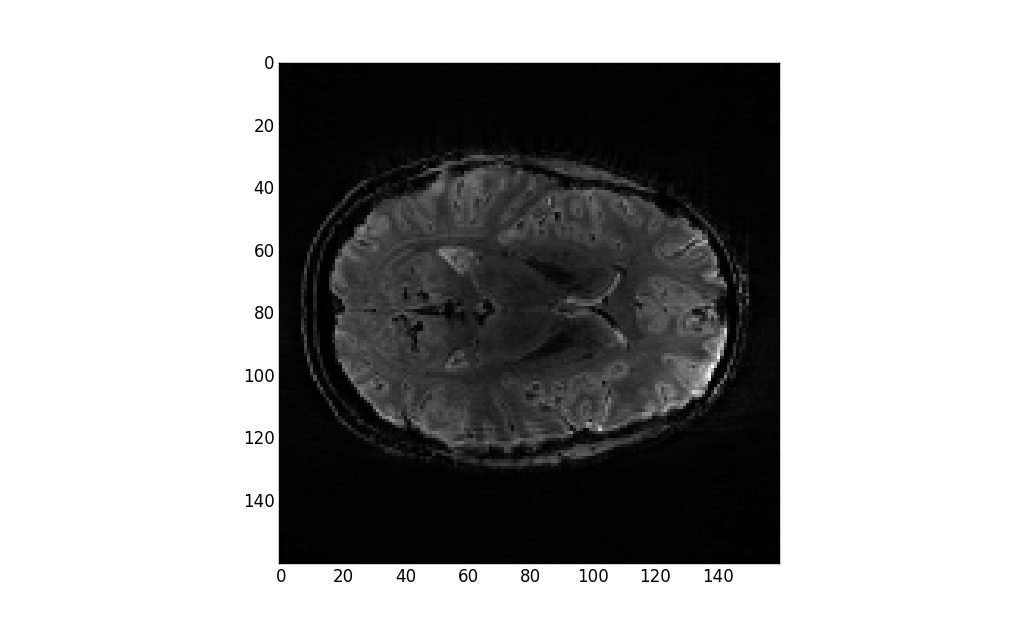
\includegraphics[scale=.5]{image_2}
\centering
\end{figure}
\begin{figure}[h]
\caption{Images below is motion and distortion corrected and have been
anatomically
aligned to a BOLD group template image that was generated from the entire group
of participants}
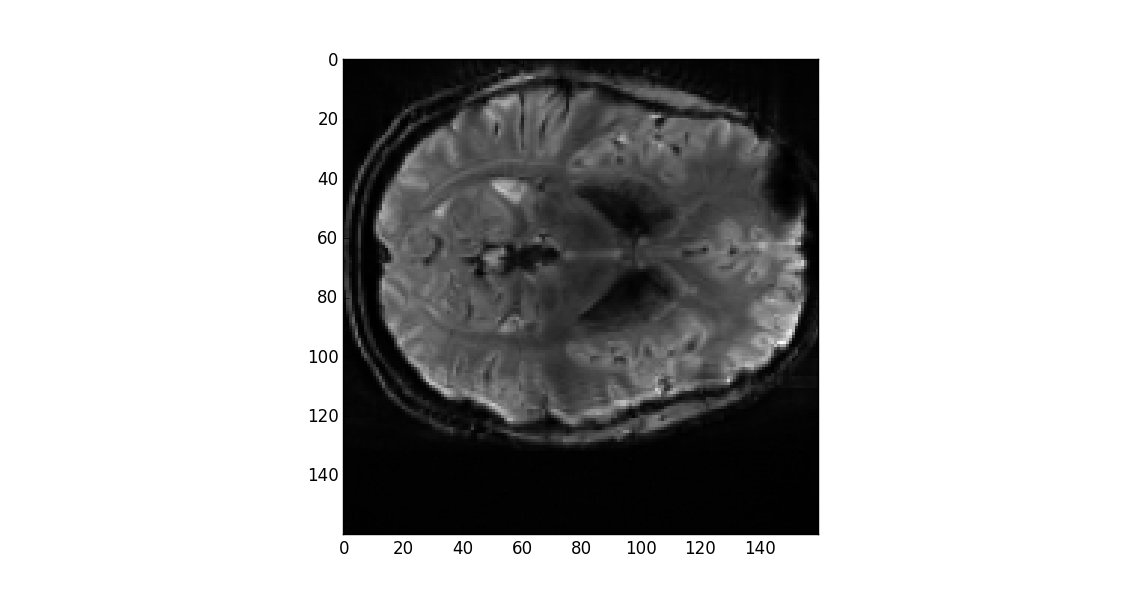
\includegraphics[scale=.5]{image_3}
\centering
\end{figure}
\begin{figure}[h]
\caption{High resolution image in NIfTI format recorded with a Philips MR
scanner at 3 Tesla using a 3D TFE sequence}
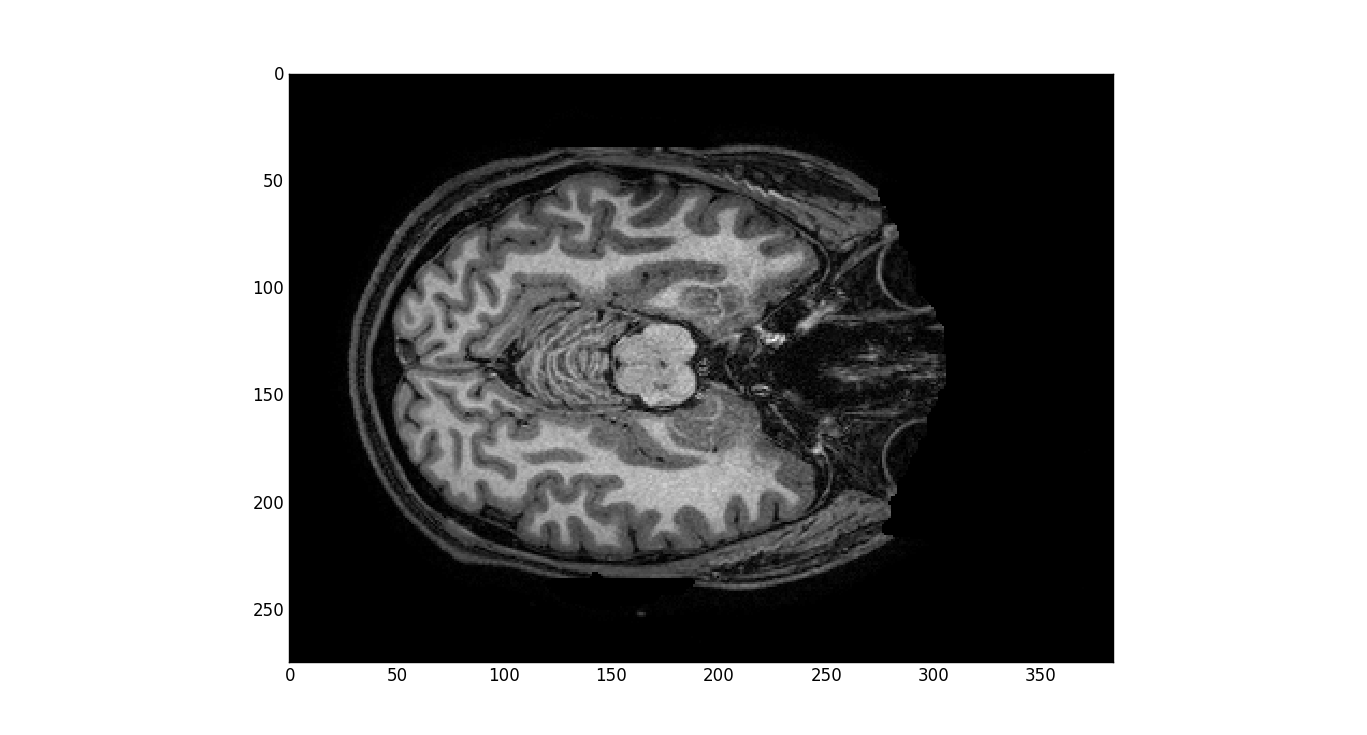
\includegraphics[scale=.4]{image_4}
\centering
\end{figure}

\bibliography{project}

\end{document}
